\documentclass{../source/Experiment}

\major{信息工程}
\name{}
\title{集成运算放大器应用电路研究}
\stuid{}
\college{信息与电子工程学院}
\date{\today}
\lab{东4-216}
\course{电子电路设计实验}
\instructor{李锡华、施红军、叶险峰}
\grades{}
\expname{集成运算放大器应用电路研究}
\exptype{研究实验}
\partner{}

\begin{document}
    \makecover
    \makeheader

    \section{实验目的}
        \begin{enumerate}
            \item 研究由集成运放构成的比例、加法、减法等基本运算电路的组成与功能,加深对集成运放线性应用电路结构和性能特点的理解,掌握其设计方法。
            \item 研究放大电路增益带宽积与单位增益带宽的关系。
            \item 了解运算放大器构成的基本运算电路在实际应用时的局限性和应考虑的问题。
        \end{enumerate}
    \section{实验任务和要求}
        \subsection{反相放大器的设计研究}
            \begin{enumerate}
                \item 设计一反相放大电路,要求Ri=10K Ω,| Av|=10。
                \item 安装该电路,加1kHz正弦信号,研究输入、输出	信号的幅度、相位关系。输入信号幅度自定。
            \end{enumerate}
            \subsubsection{数据记录要求}
                \begin{enumerate}
                    \item 电路图、元件值	
                    \item 一组直流:双踪示波,一幅图 + 数据说明(DC耦合,输出不饱和)
                    \item 两组交流:A. 无衰减:一幅图 + 数据说明(AC耦合即可,输出不失真)\\ B. 40dB衰减:仅数据
                \end{enumerate}
        \subsection{设计并安装一个算术运算电路}
                要求实现:\\
                A、$Vo = -(V_{i1}+0.5V_{i2})$ \\
                B、$Vo = V_{i1}-V_{i2}$ \\
                A、B选做一个 \\
                Vi1用直流、Vi2用正弦信号在合适的幅度和频率范围内,进行验证并记录波形及参数。
                \subsubsection{数据记录要求}
                \begin{enumerate}
                    \item 电路图、元件值	
                    \item 一组数据:双踪示波,一幅图 + 数据说明(DC耦合,输出不失真)
                    \item 仿真并比较:内容  Trans
                    *实验报告必须有手绘坐标草图、数据说明要完整(如周期、直流分量、幅度等必要参数),结果、与设计比较。可以没有拍照图
                \end{enumerate}
        \subsection{增益带宽积研究}
        研究所给电路下不同Rf时的带宽积。填下表。
        \begin{table}[h]
            \centering
            \begin{tabular}{|c|c|c|c|c|c|}
            \hline
            \multicolumn{2}{|c|}{$R_f$} & $R_1$       & $A_v$ & $BW$     & $A_v \dot BW$ \\ \hline
            1       & $10k\Omega$       & $10k\Omega$ &      &  &       \\ \hline
            2       & $100k\Omega$      & $10k\Omega$ &     &   &       \\ \hline
            3       & $1M\Omega$        & $10k\Omega$ &   &  &    \\ \hline
            \end{tabular}
            \caption{增益带宽积研究}
            \end{table}
    \section{实验方案设计与实验参数计算}
        \subsection{反相放大器}
        电路图如下:
            \begin{figure}[h]
                \centering
                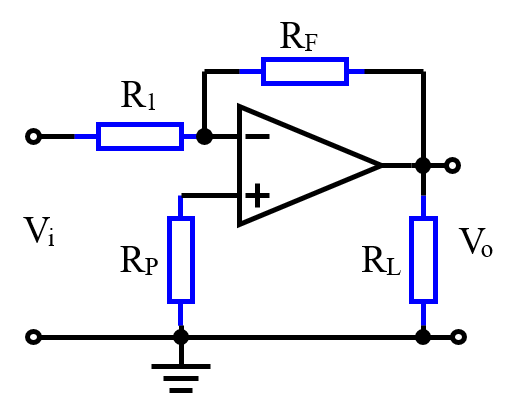
\includegraphics[width = 3in]{运算2}
                \caption{电路图}
            \end{figure}
        由$$A_v = -\frac{R_F}{R_1}$$
        所以取$Rf = 100k\Omega$、$R_1 = 10k\Omega$,同时取$R_P = 0\Omega$
        \subsection{算数运算电路}
        我们小组选择A\\
        设计电路图如下:
            \begin{figure}[h]
                \centering
                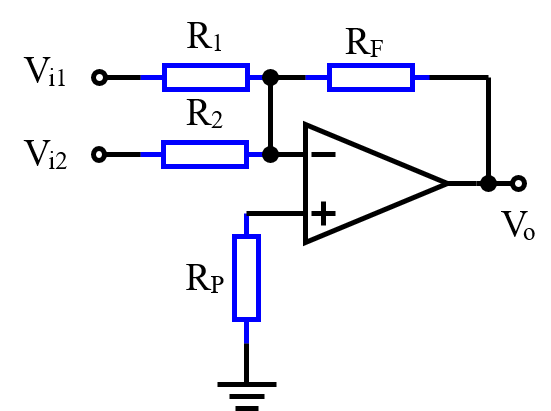
\includegraphics[width = 3in]{运算3}
                \caption{电路图}
            \end{figure}
        由反向权重加法器中:
        $$V_o = -(\frac{R_F}{R_1}V_{i1}+\frac{R_F}{R_2}V_{i2})$$
        选取$R_F = 100k\Omega$,则$R_1 = 100k\Omega$、$R_2 = 10k\Omega$,同时取$R_P = 0\Omega$
    \section{主要仪器设备}
    电路板、信号发生器、示波器、直流电源
    \section{实验步骤、实验调试过程、实验数据记录}
        \subsection{反相放大器}
        电路图:
        \newpage
        \begin{figure}[h]
            \centering
            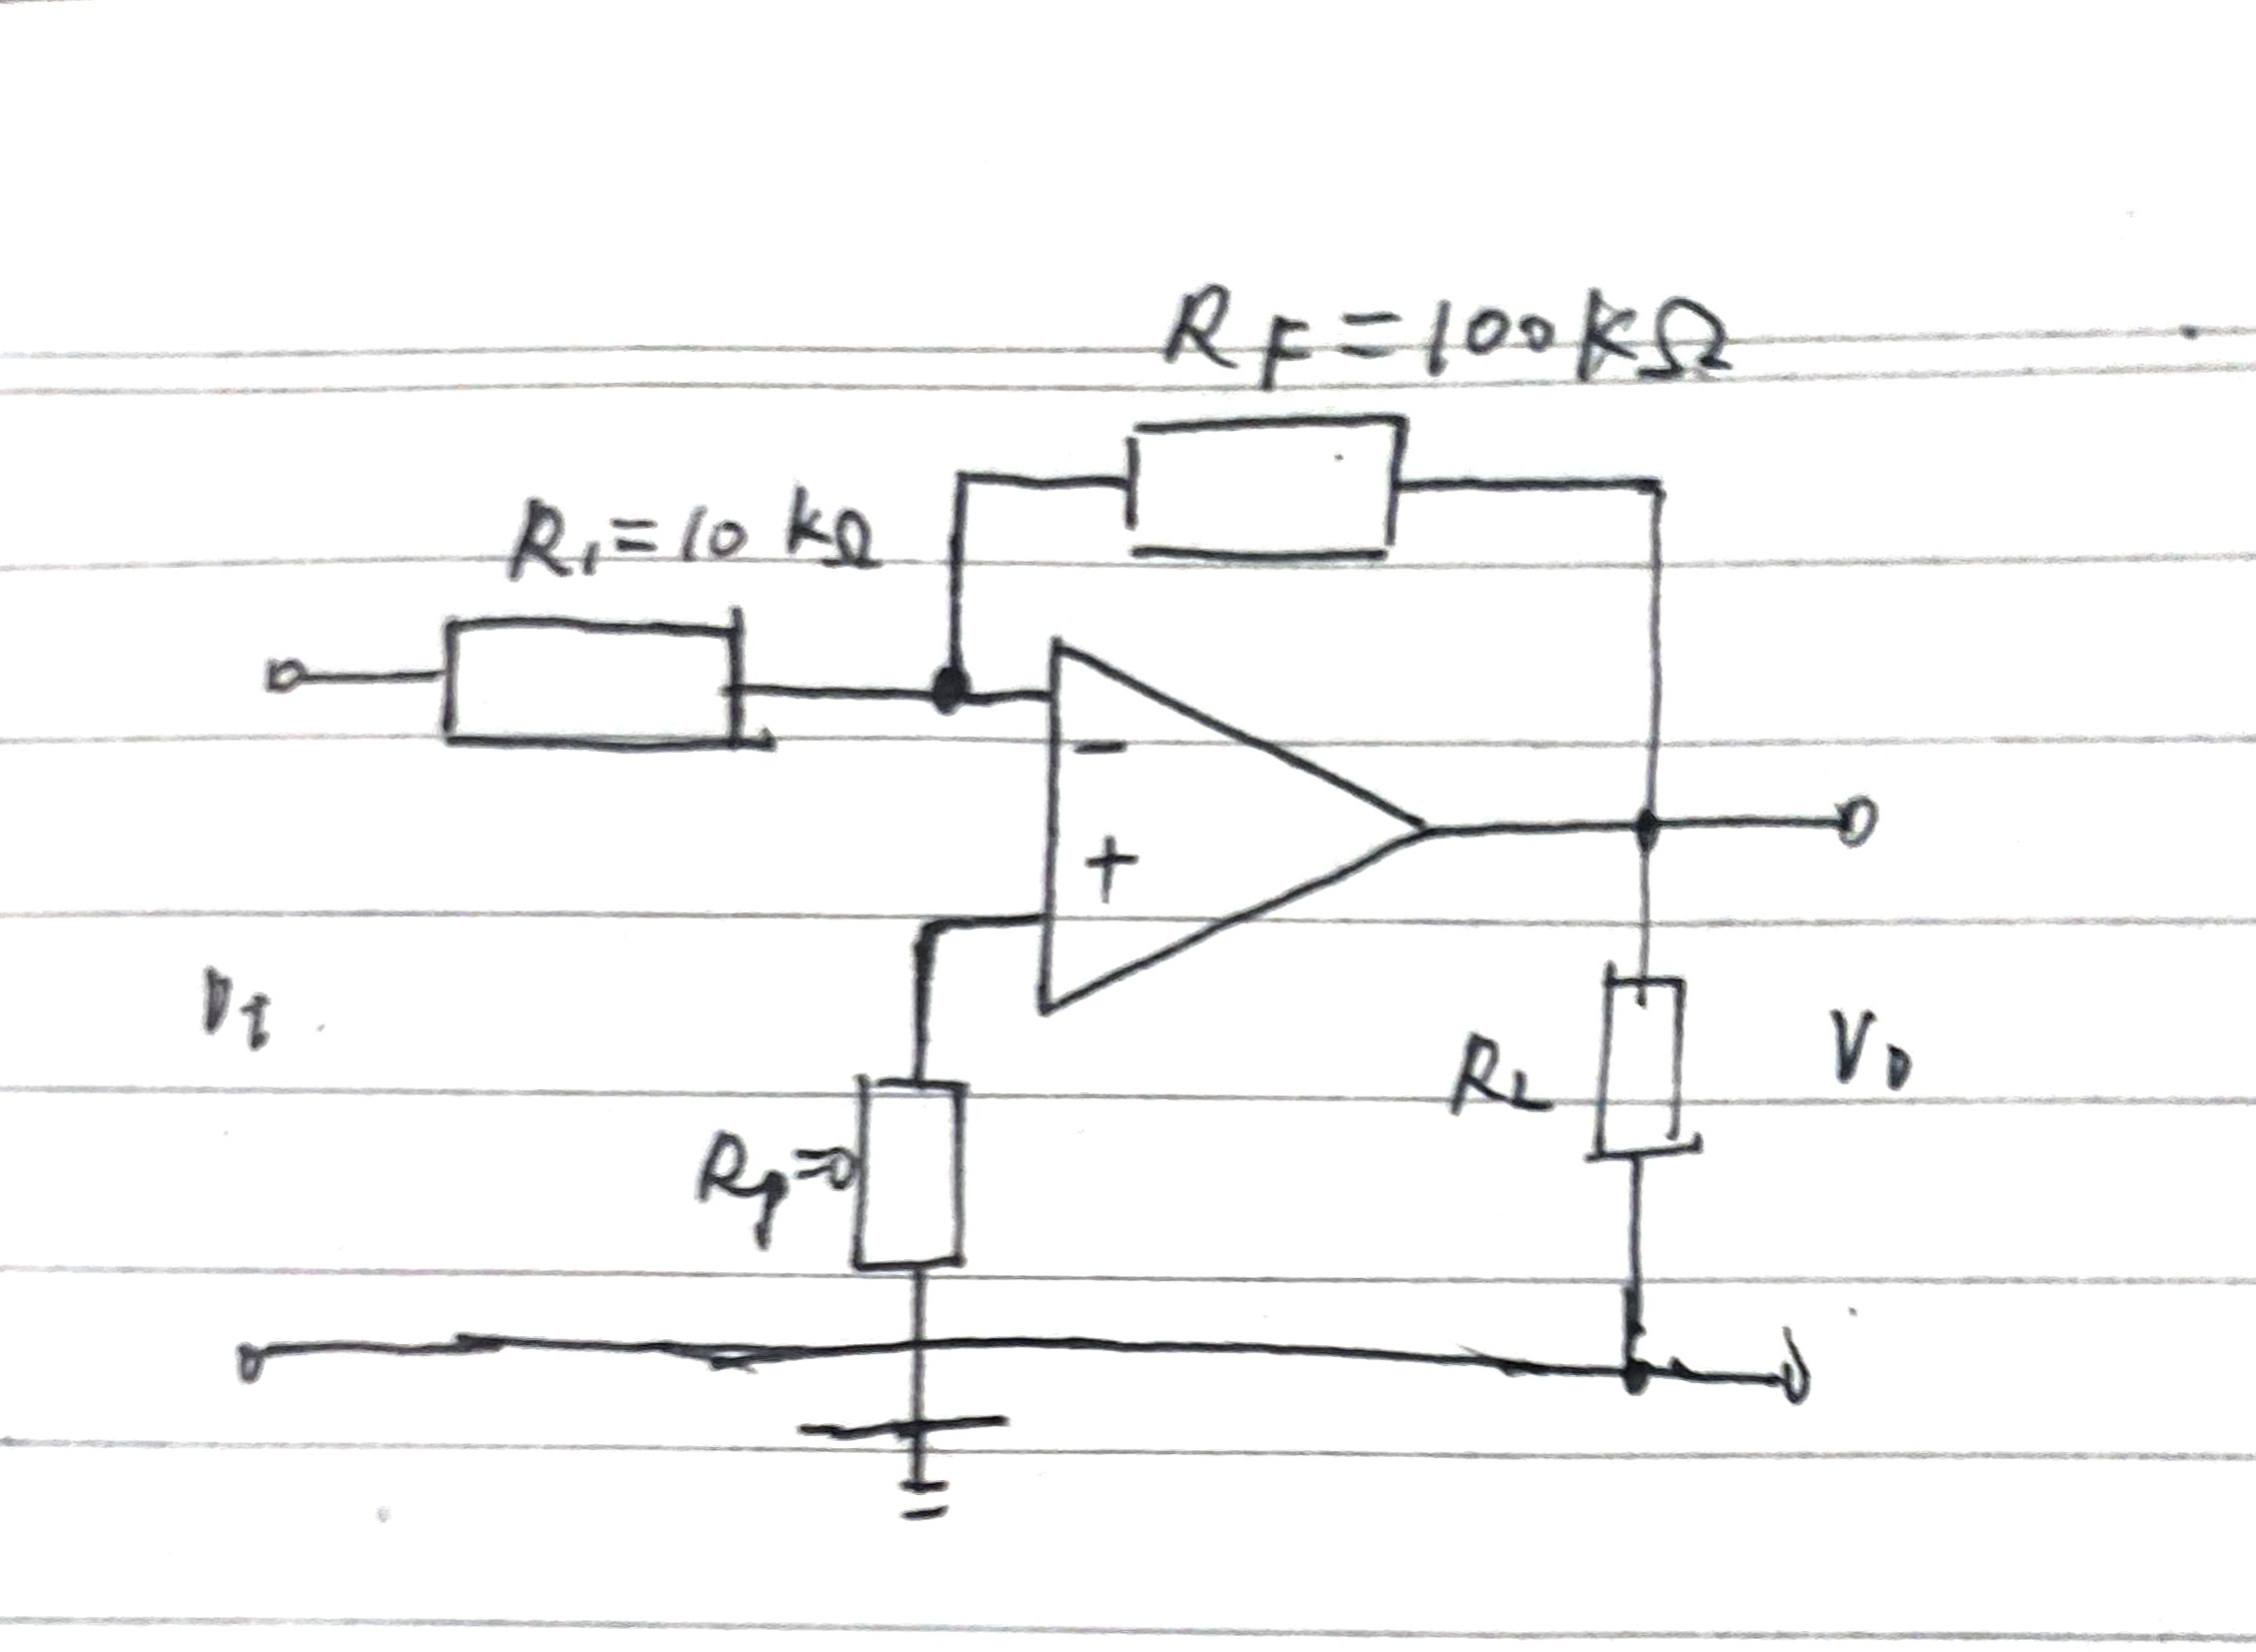
\includegraphics[width = 3in]{运算4}
            \caption{电路图}
        \end{figure}
        元件值:
        $Rf = 100k\Omega,\,R_1 = 10k\Omega,\,R_P = 0\Omega$\\
        结果如下:
        \begin{figure}[h]
            \centering
            \subfigure[1]{
                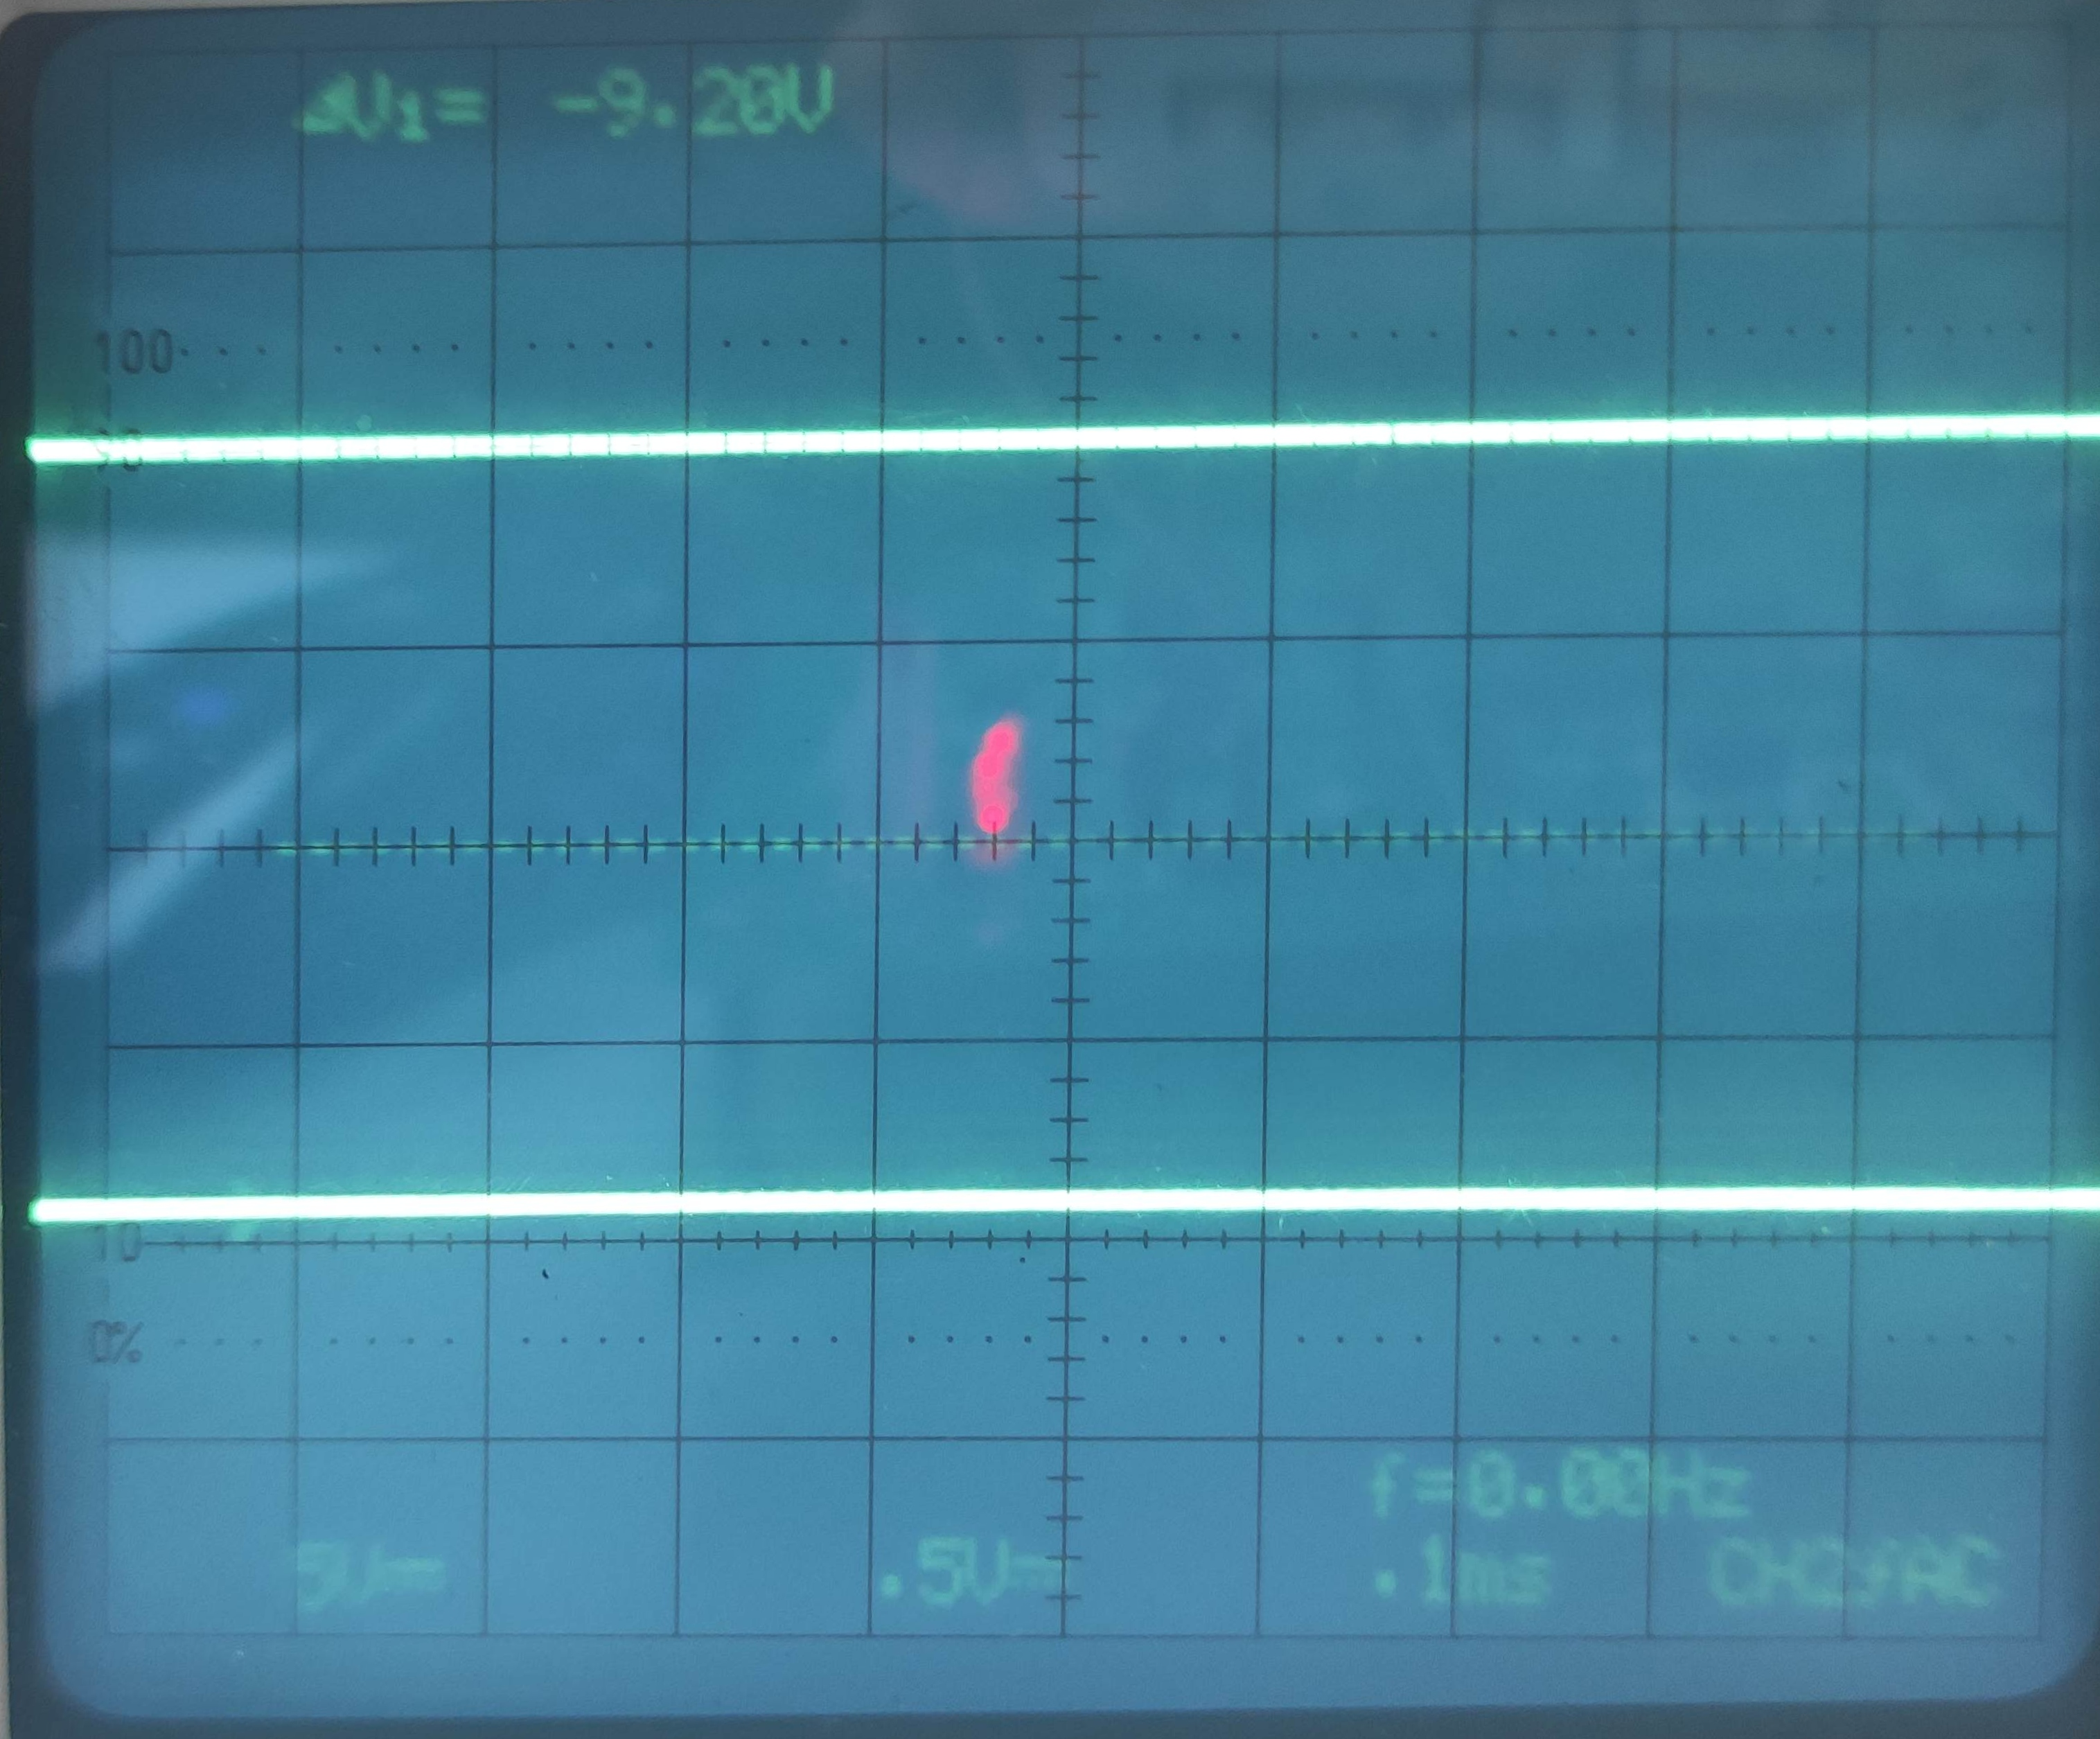
\includegraphics[width = 3in]{运算6}
            }
            \subfigure[2]{
            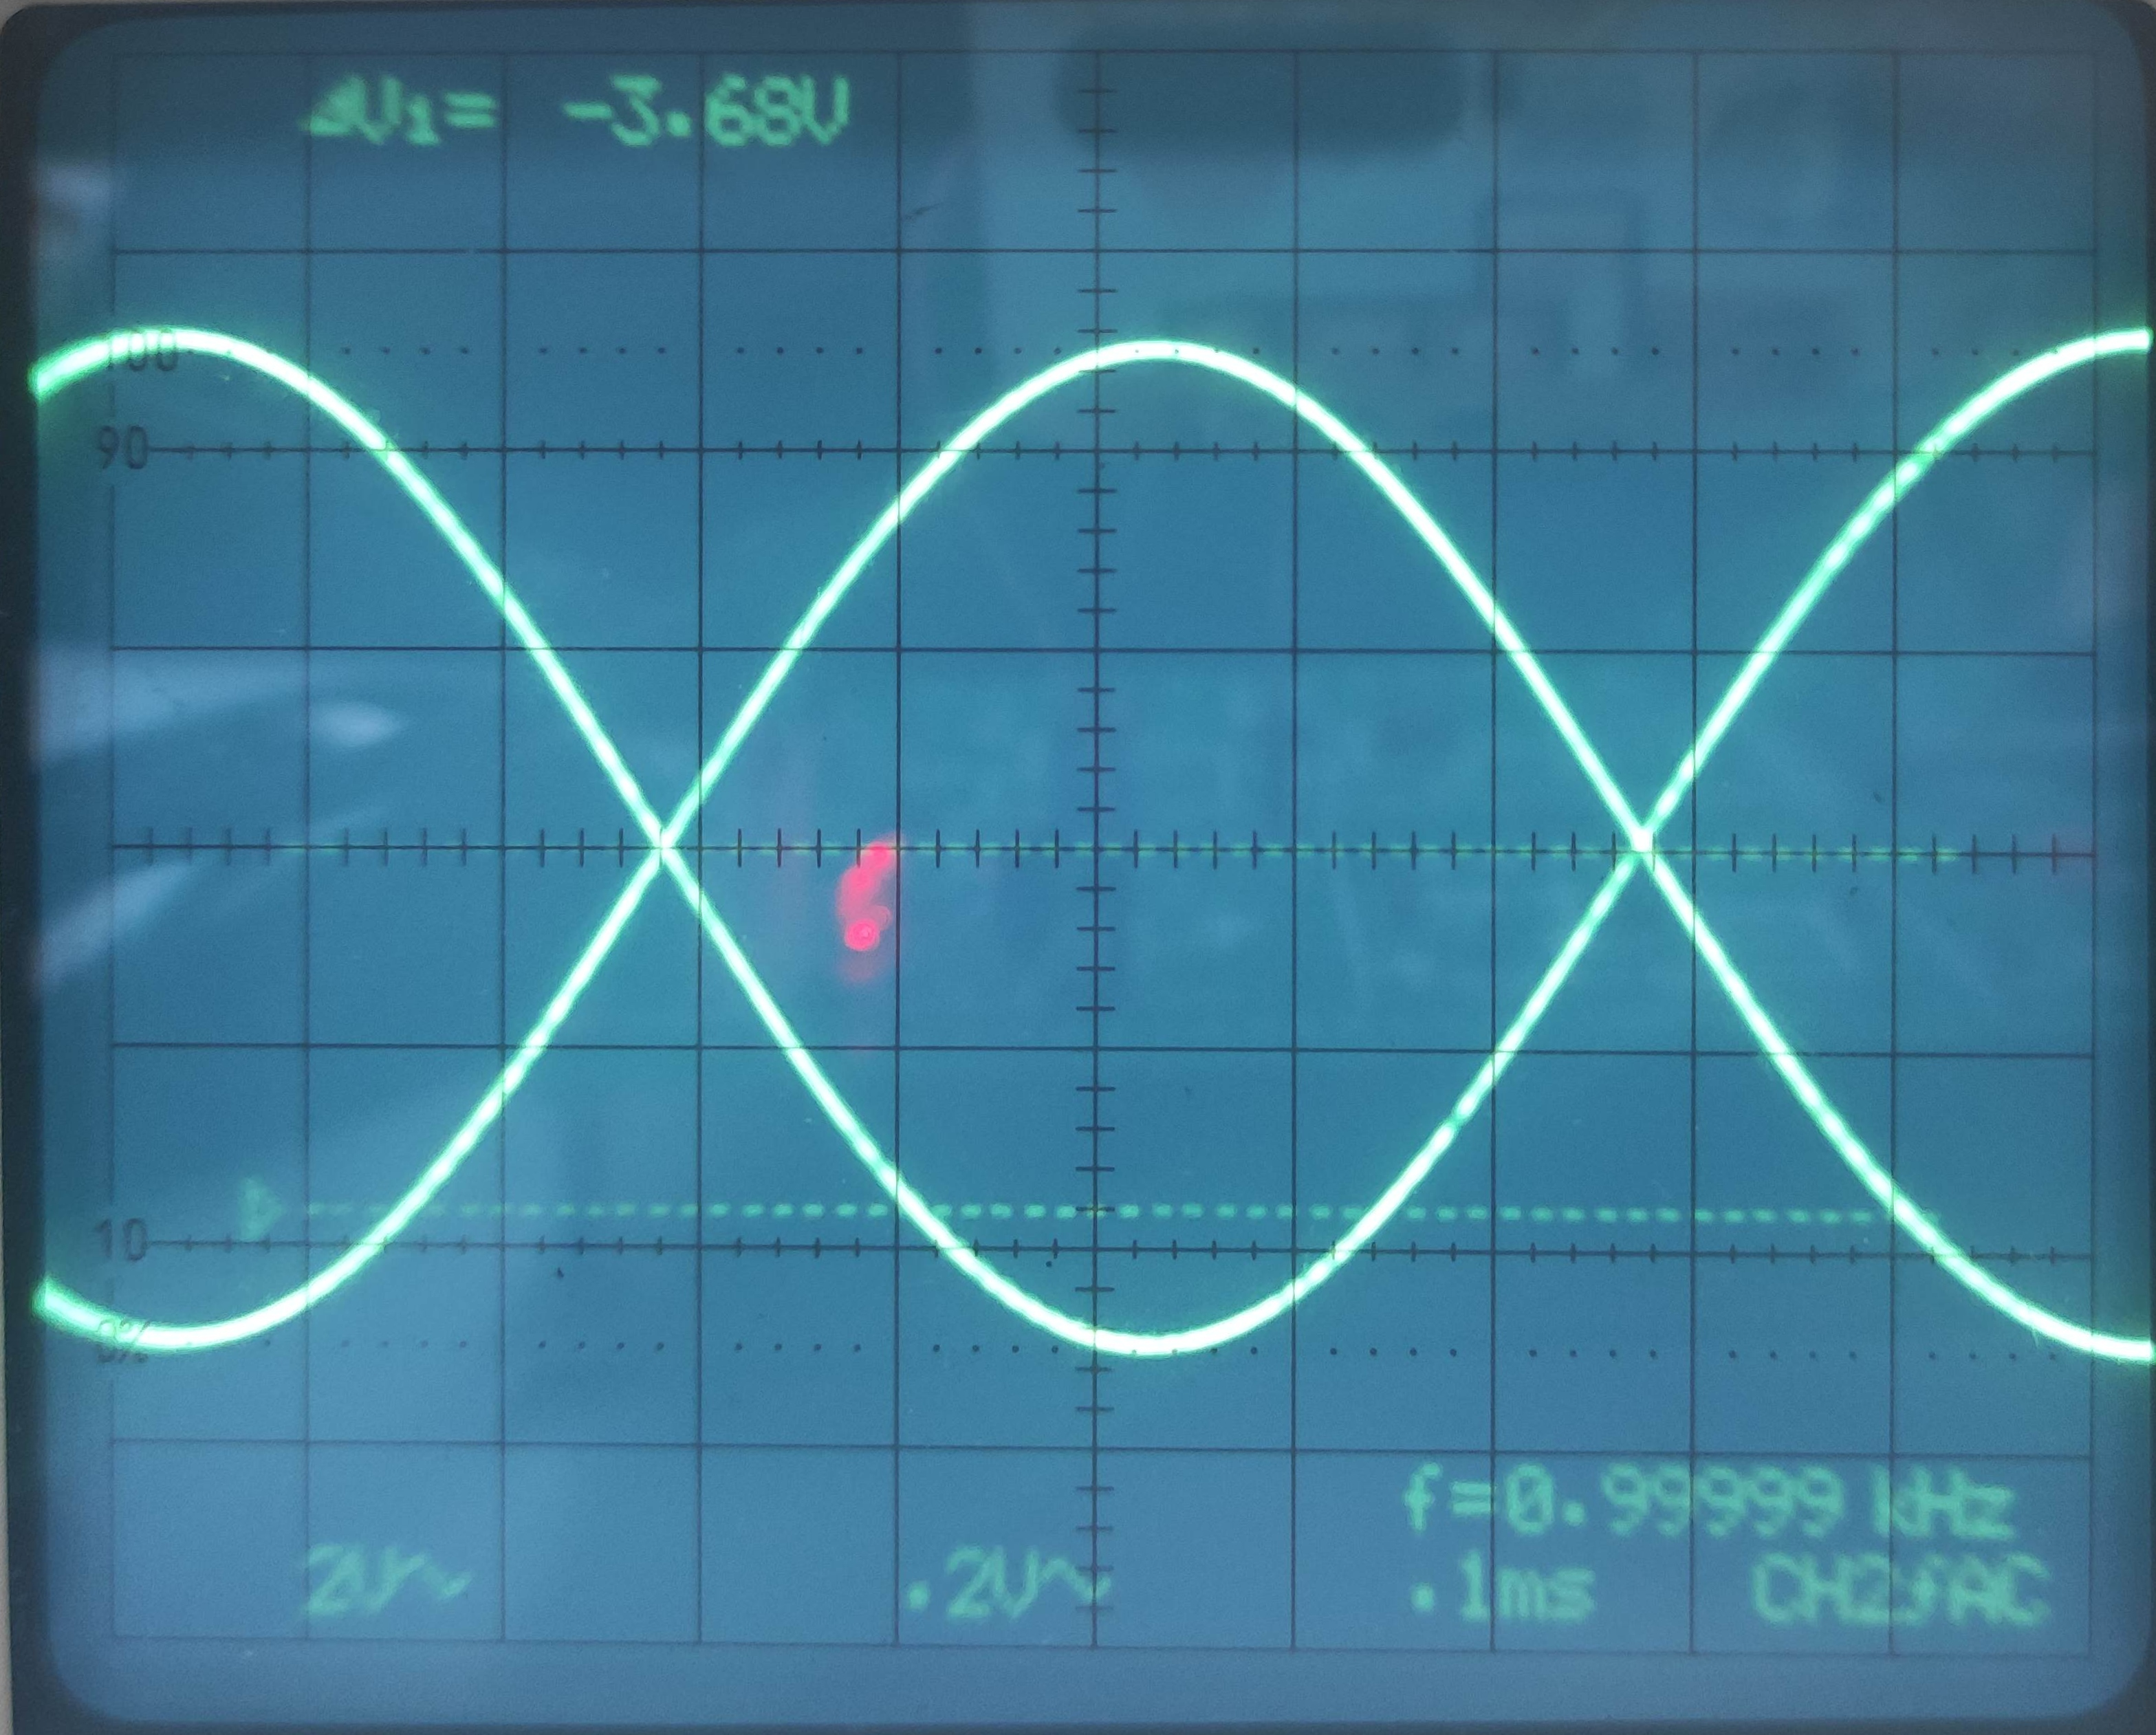
\includegraphics[width = 3in]{运算7}
            }
            \caption{直流和交流耦合图}
        \end{figure}
        \newpage
        \begin{table}[h]
            \centering
            \begin{tabular}{|c|c|c|}
            \hline
            $V_i$ & $V_o$   & $A_v$ \\ \hline
            $1V$  & $9.20V$ & 9.20  \\ \hline
            \end{tabular}
            \caption{直流结果}
            \begin{tabular}{|c|c|c|c|}
            \hline
            \multicolumn{2}{|c|}{$V_i$} & $V_o$   & $A_v$ \\ \hline
            1         & $0.52V$         & $5.12V$ & 9.85  \\ \hline
            2         & $55.1mV$        & $552mV$ & 10.02 \\ \hline
            \end{tabular}
            \caption{交流结果}
            \end{table}
            \subsection{算术运算器}
            电路图:
            % \newpage
            \begin{figure}[h]
                \centering
                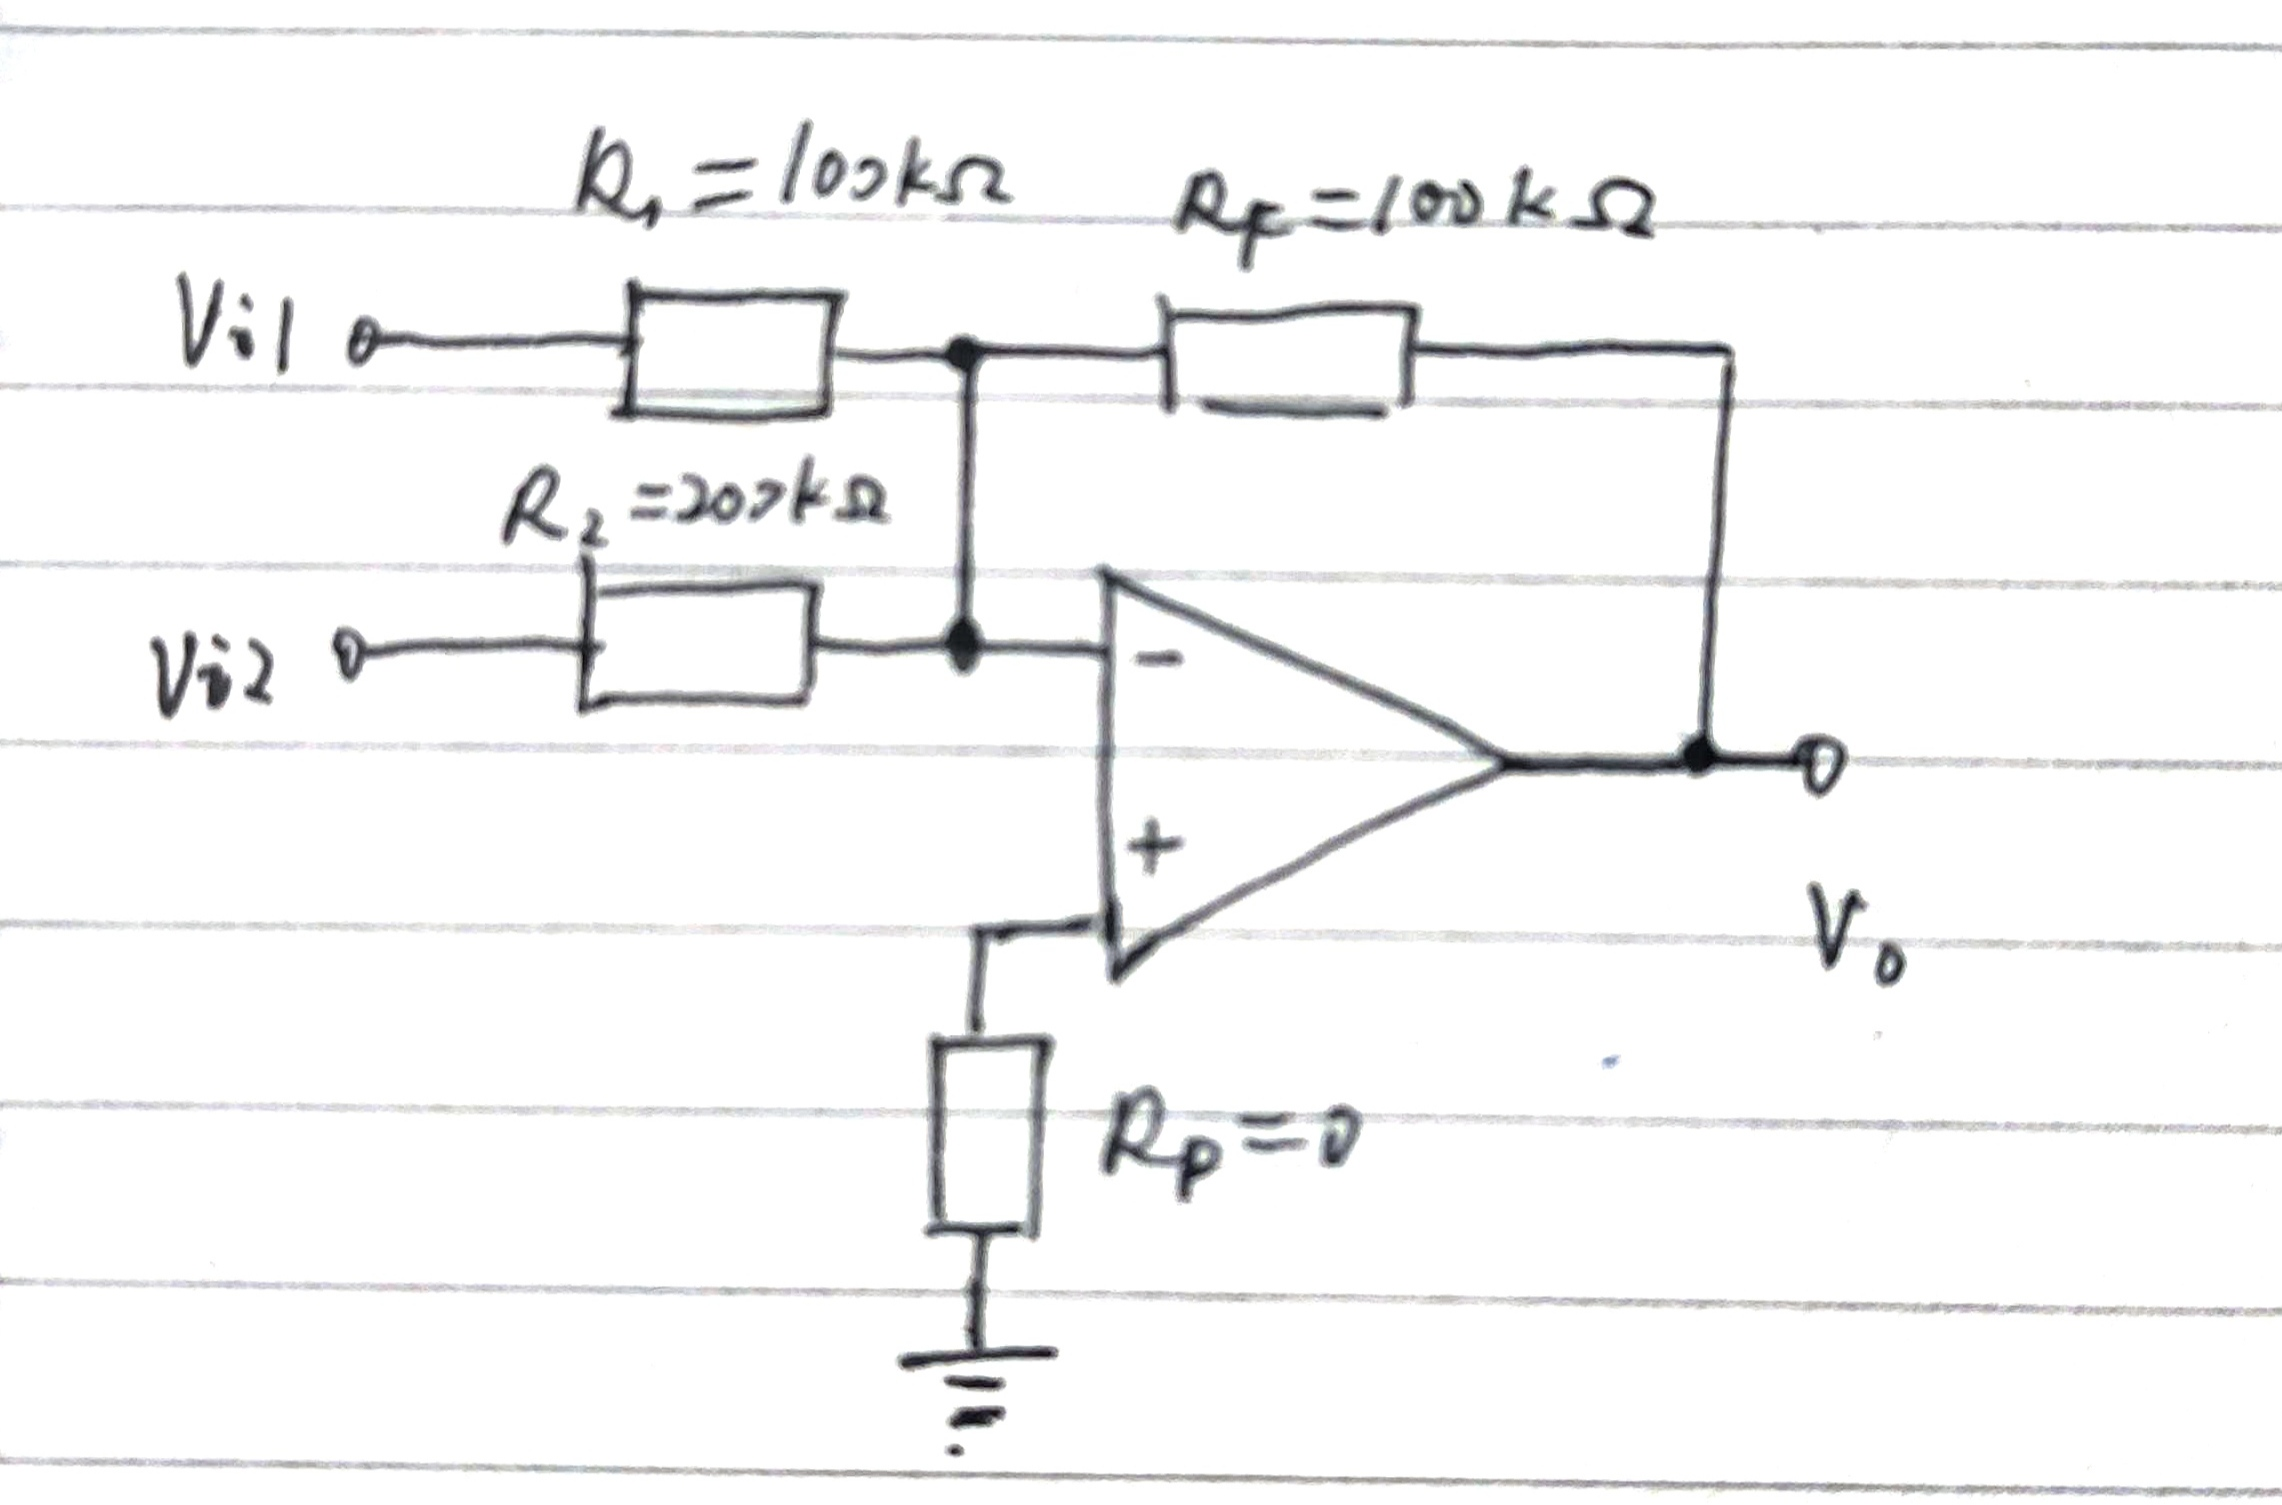
\includegraphics[width = 3in]{运算5}
                \caption{电路图}
            \end{figure}
            元件值:
            $Rf = 100k\Omega,\,R_1 = 100k\Omega,\,R_2 = 200k\Omega,\,R_P = 0\Omega$\\
            结果如下:\\
            % \newpage
            \begin{figure}[h]
                \centering
                \subfigure[拍照]{
                    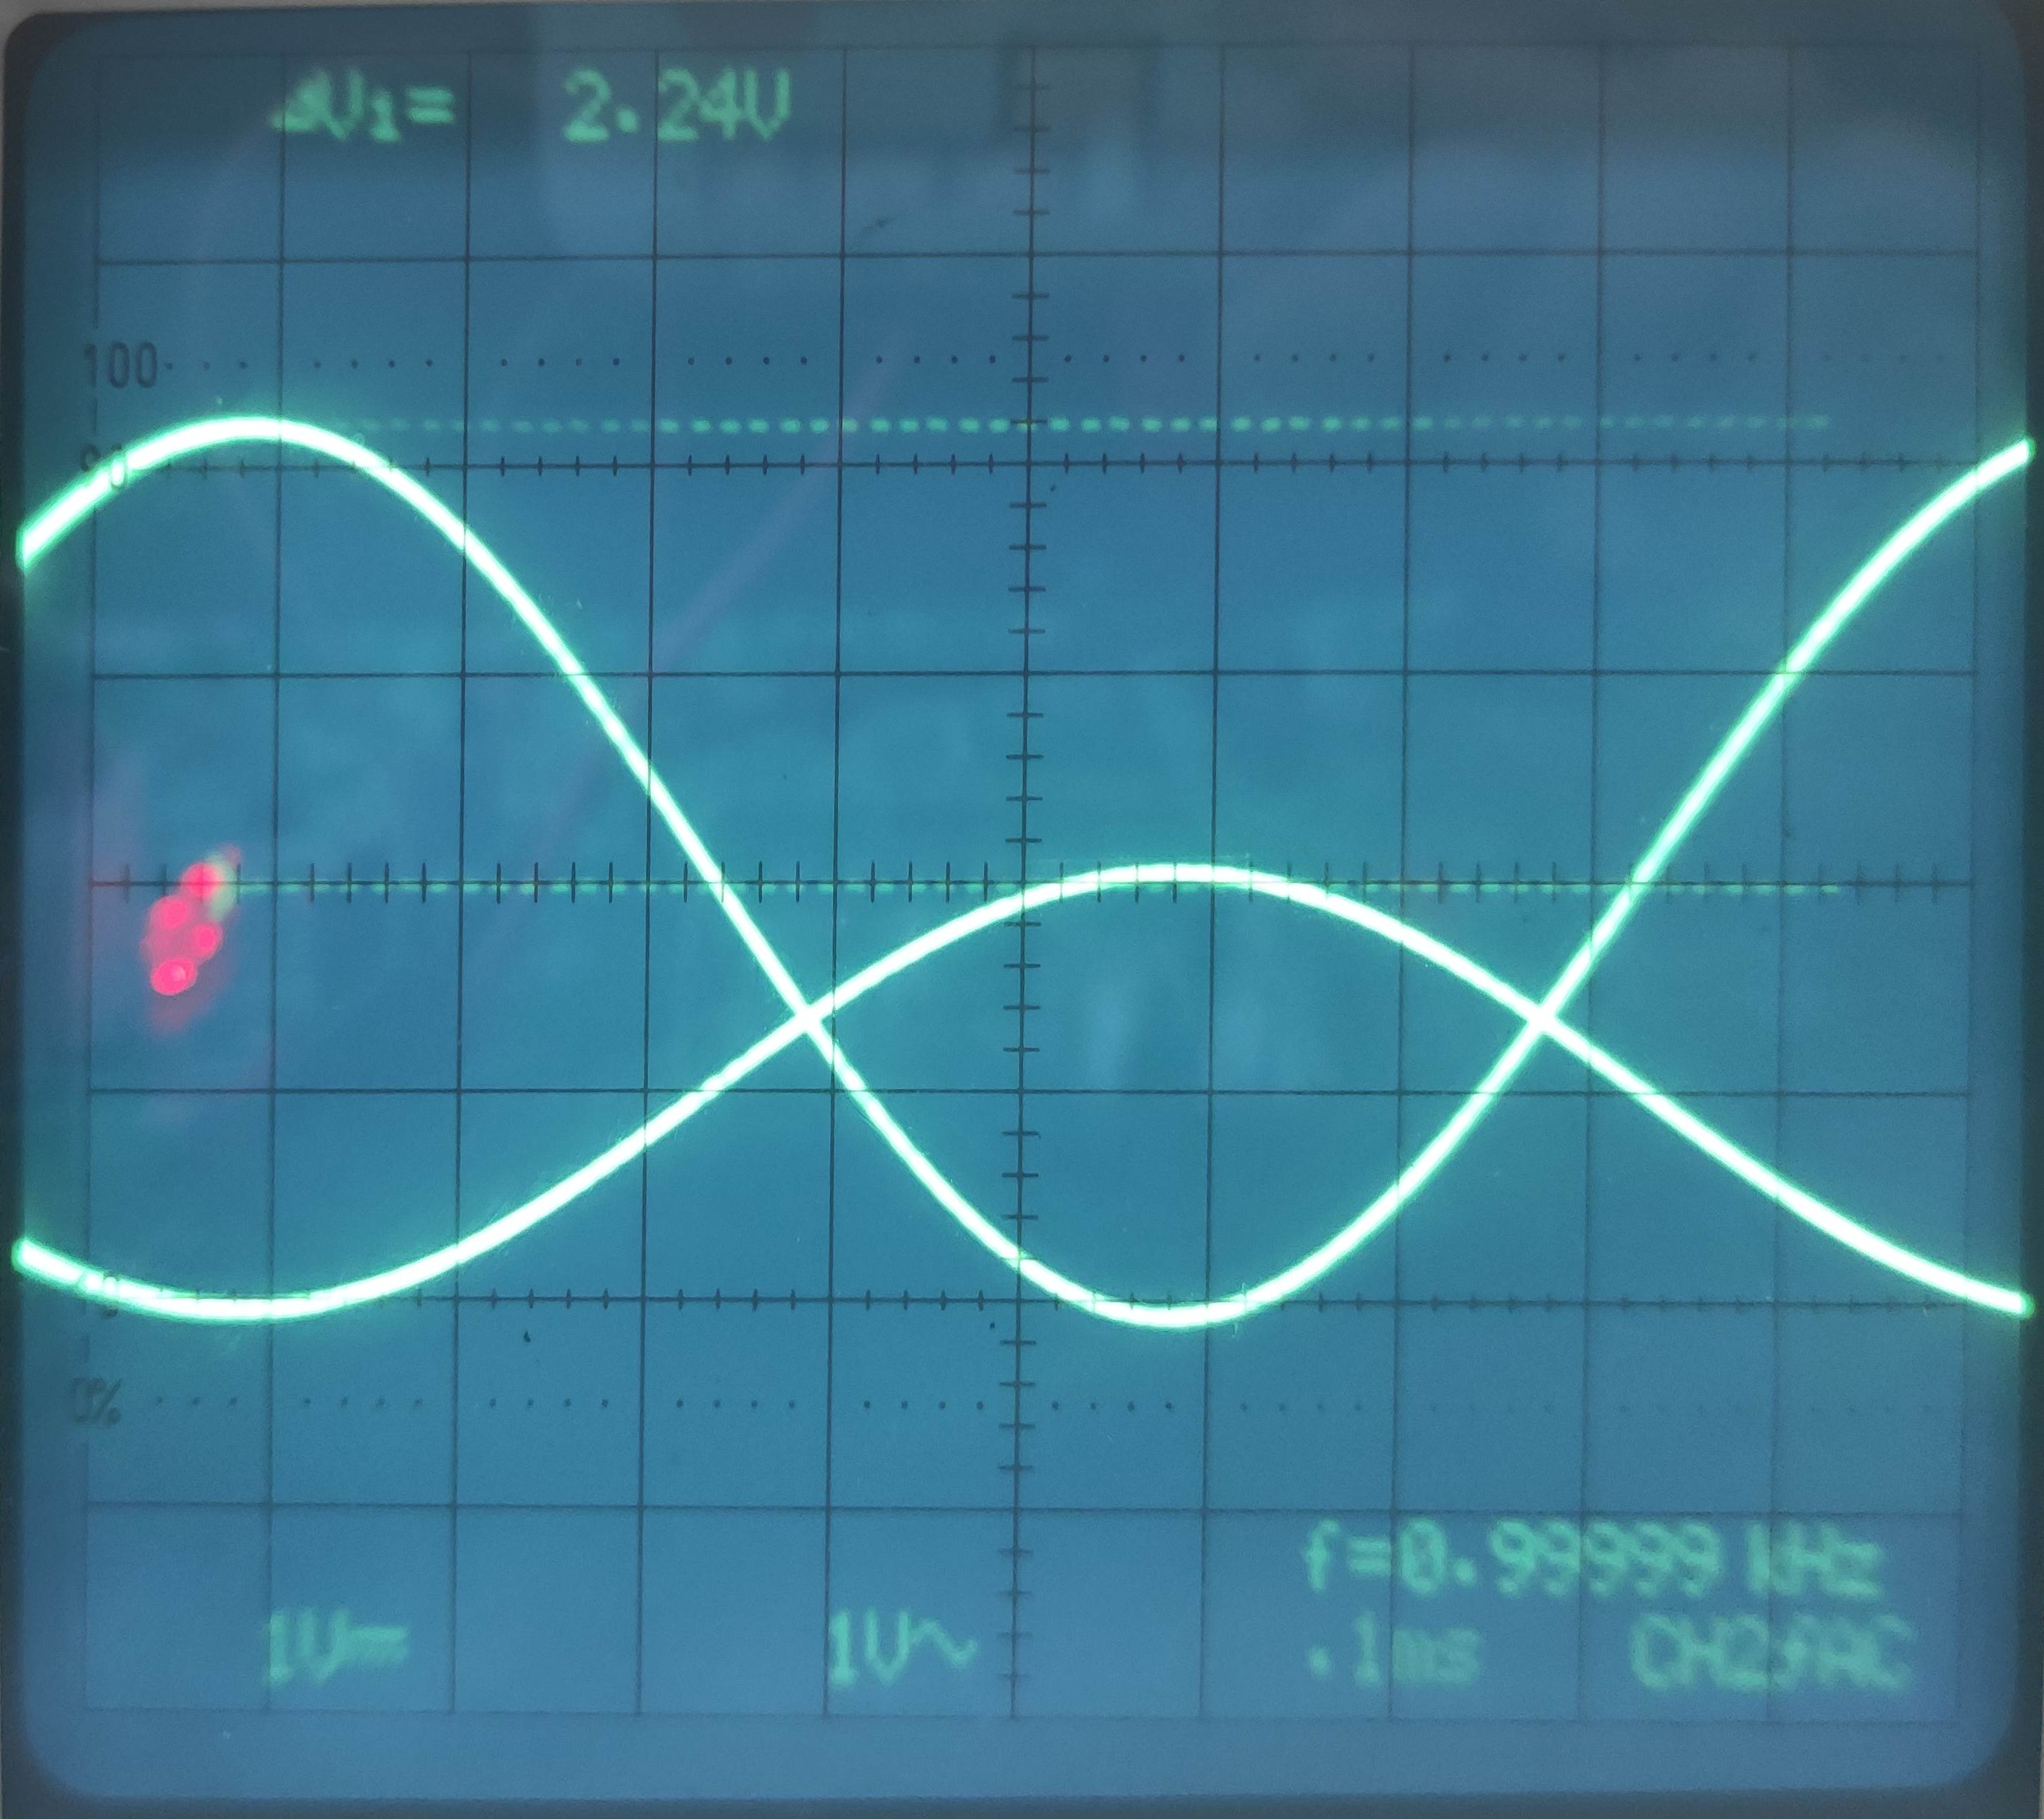
\includegraphics[width = 2in]{运算8}
                }
                \subfigure[草图]{
                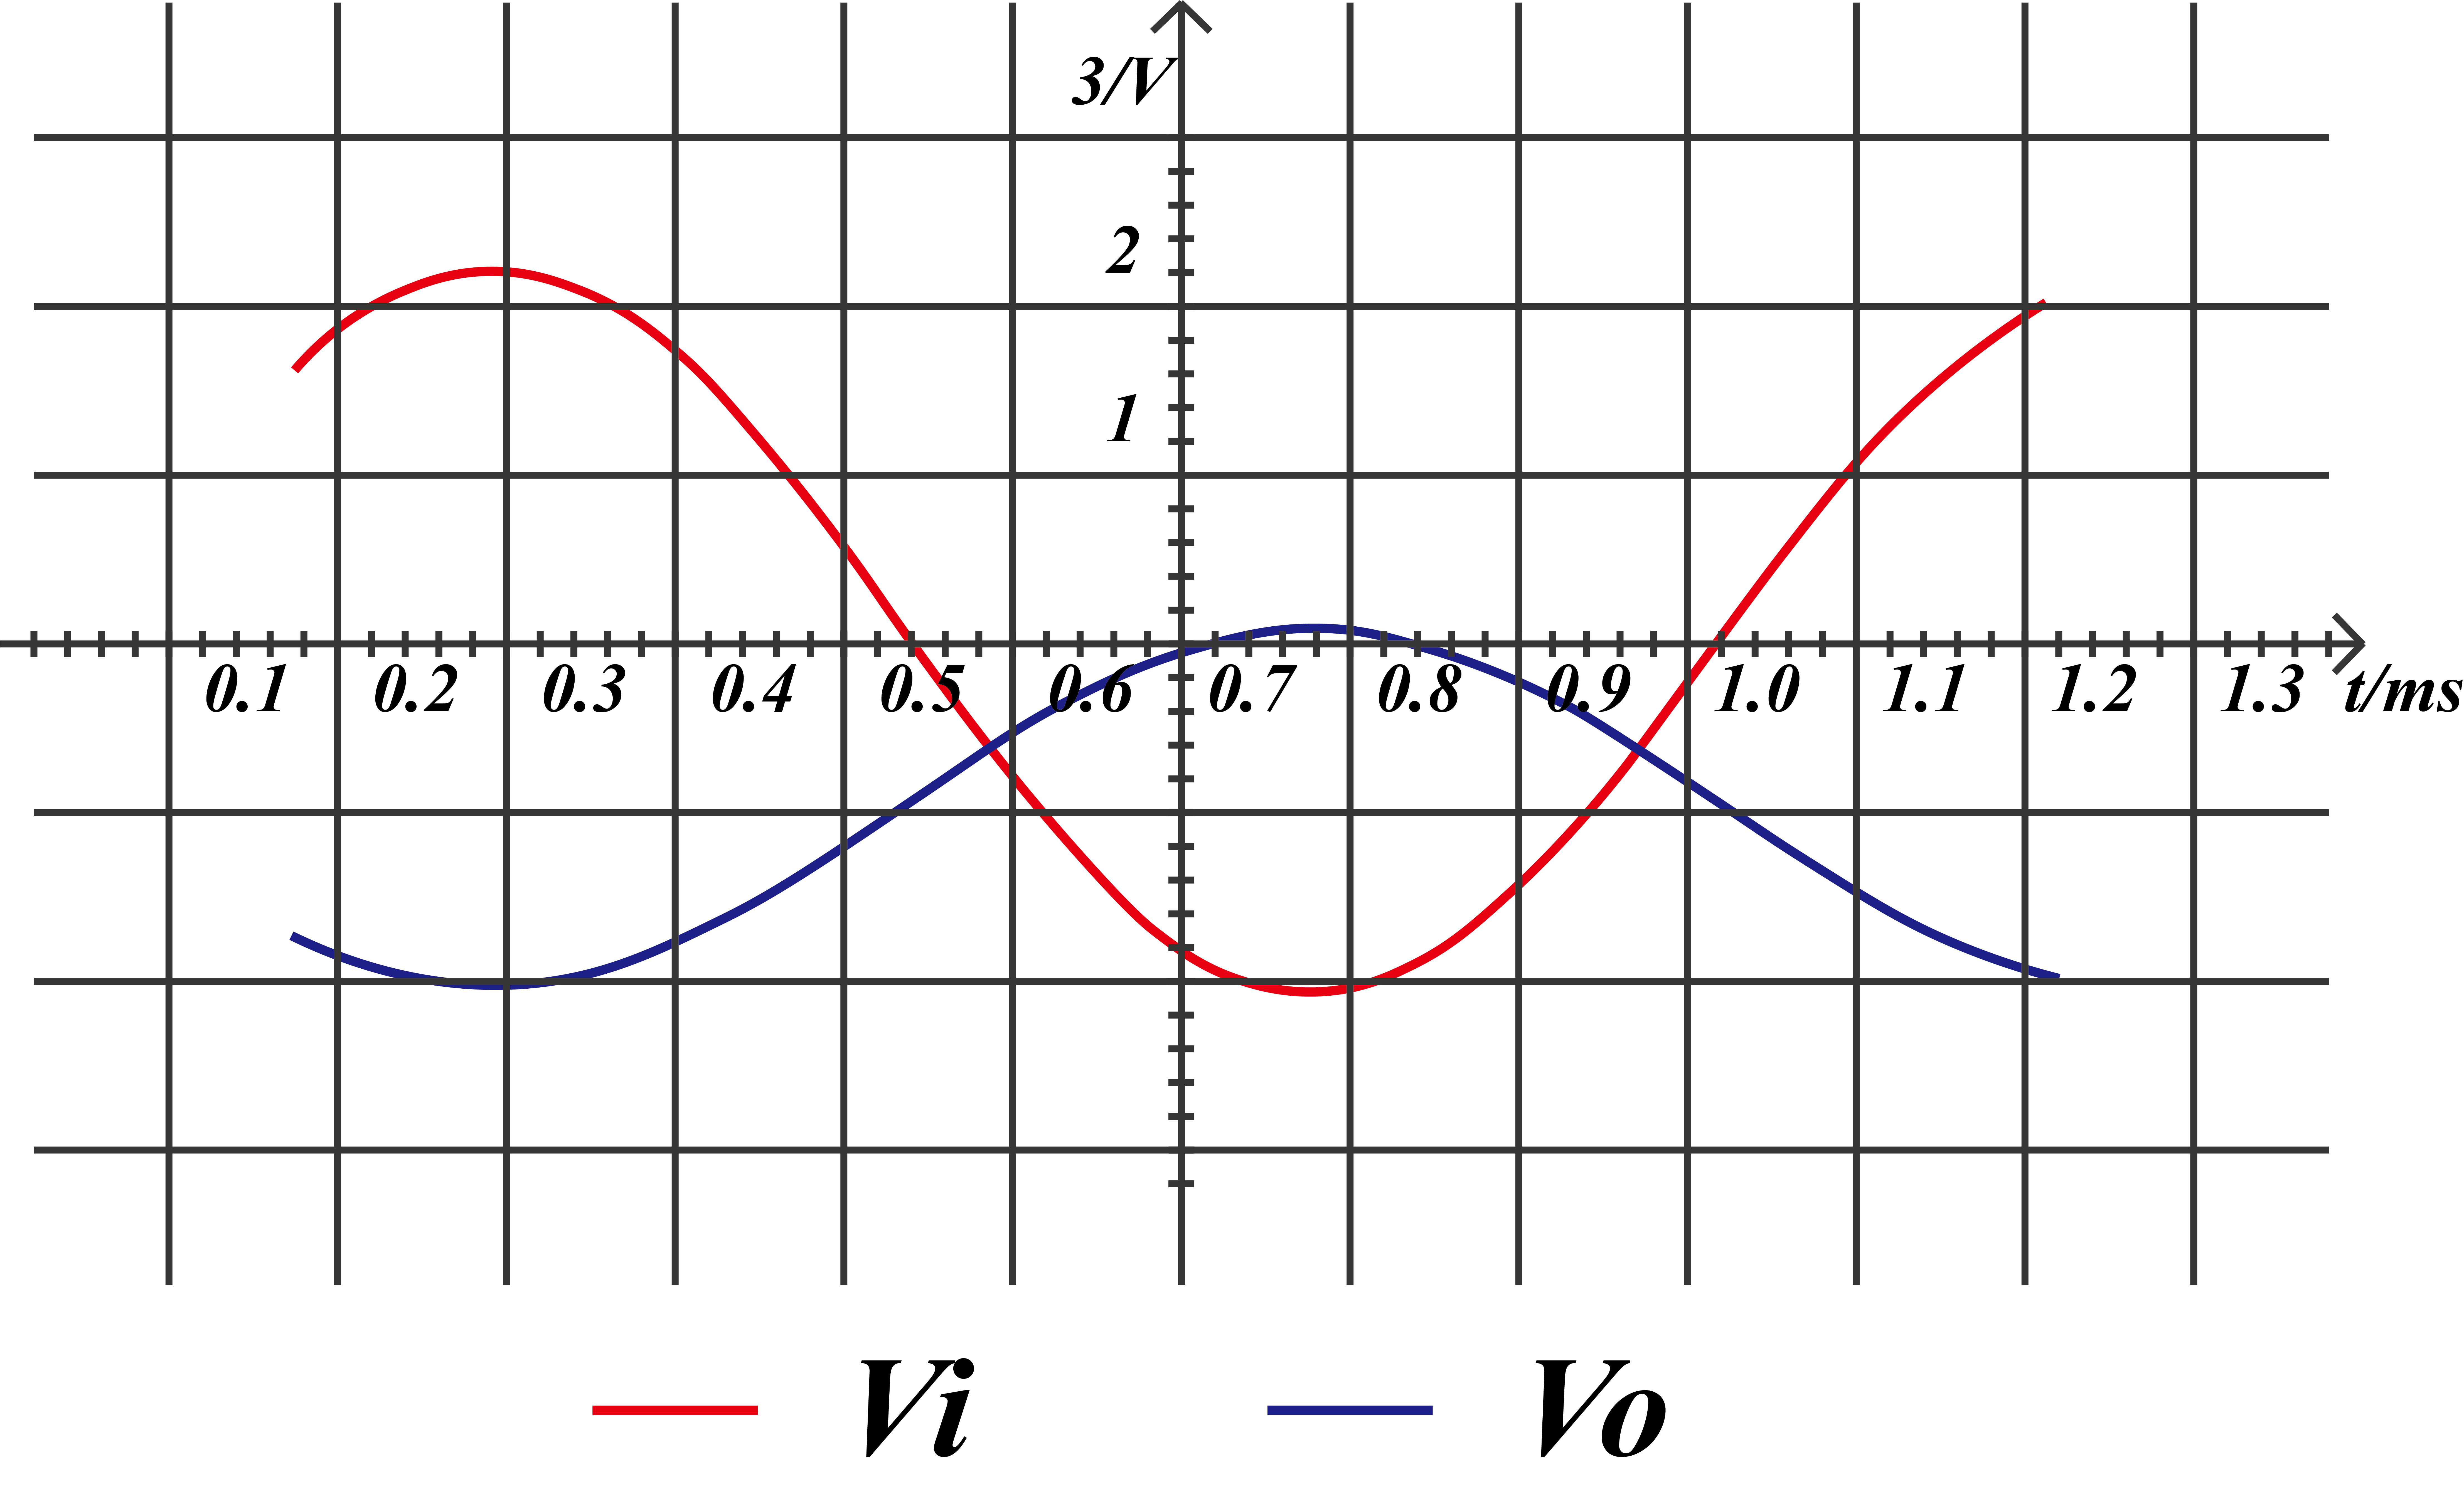
\includegraphics[width = 2.5in]{运算9}
                }
            \end{figure}
            说明:\\
            频率:$f = 1kHz$\\
            直流分量:$V_{i1} = 1V$\\
            交流分量:$V_{i2} = 4.4V$\\
            $V_o = 2.2V$ \par 
            仿真分析:\\
            \begin{figure}[h]
                \centering
                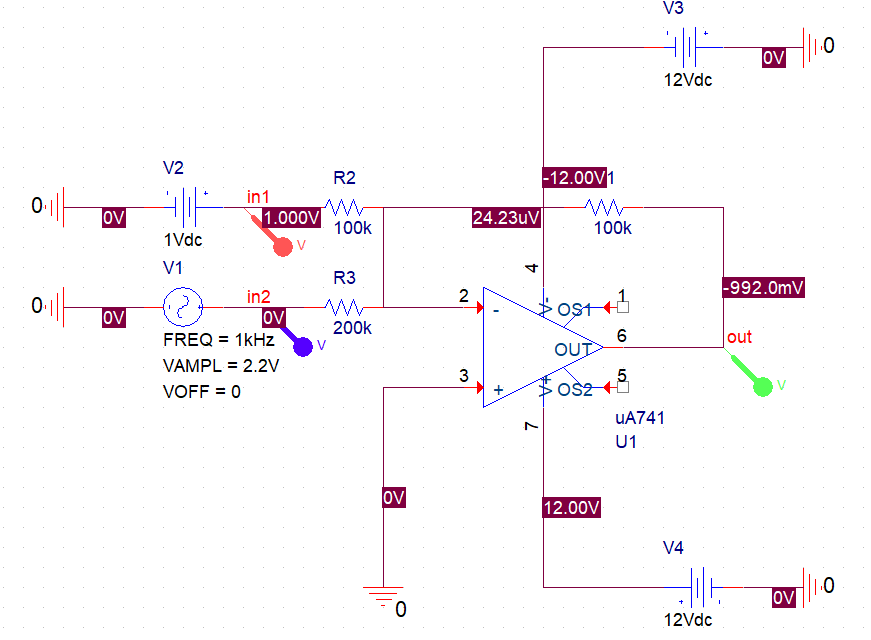
\includegraphics[width = 3.5in]{运算10}
                \caption{电路图}
                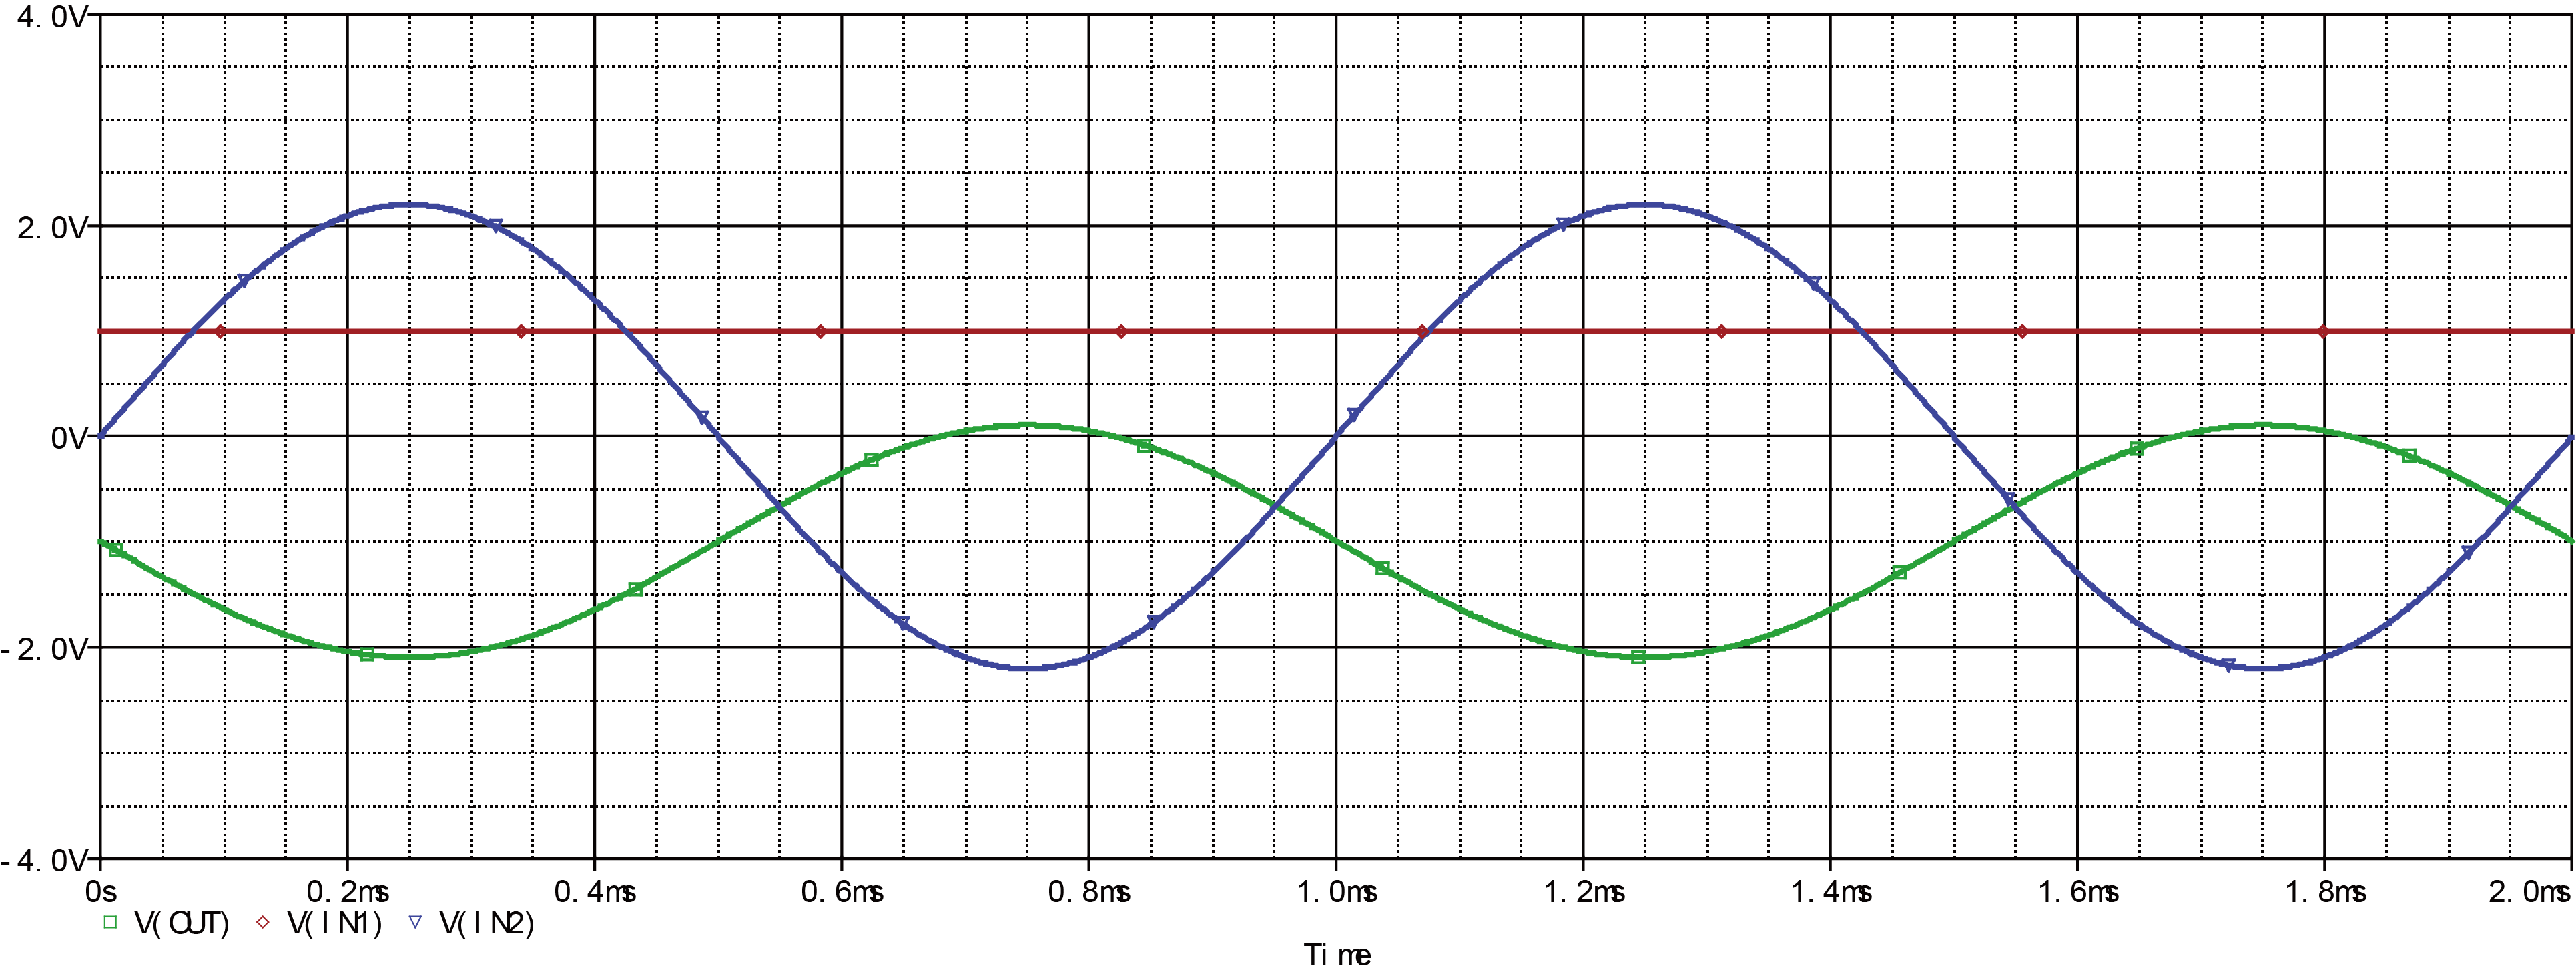
\includegraphics[width = 4in]{运算}
                \caption{仿真结果}
            \end{figure}
            \subsection{增益带宽积研究}
            电路图:
            \newpage
            \begin{figure}[h]
                \centering
                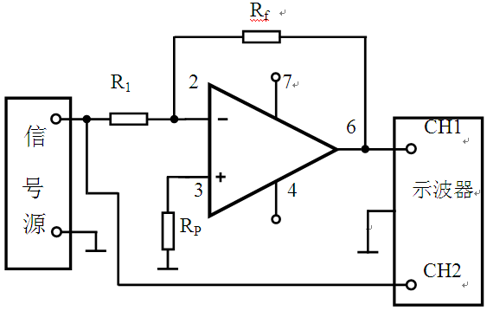
\includegraphics[width = 3in]{运算19}
                \caption{电路图}
            \end{figure}
            结果如下:
            \begin{table}[h]
                \centering
                \begin{tabular}{|c|c|c|c|c|c|}
                \hline
                \multicolumn{2}{|c|}{$R_f$} & $R_1$       & $A_v$ & $BW$     & $A_v \dot BW$ \\ \hline
                1       & $10k\Omega$       & $10k\Omega$ & 1     & $640kHz$ & $640kHz$      \\ \hline
                2       & $100k\Omega$      & $10k\Omega$ & 10    & $68kHz$  & $680kHz$      \\ \hline
                3       & $1M\Omega$        & $10k\Omega$ & 98.1  & $7.3kHz$ & $716.13kHz$   \\ \hline
                \end{tabular}
                \caption{实验结果}
                \end{table}
                \par
            仿真分析:\par
            电路图
            \newpage
            \begin{figure}[h]
                \centering
                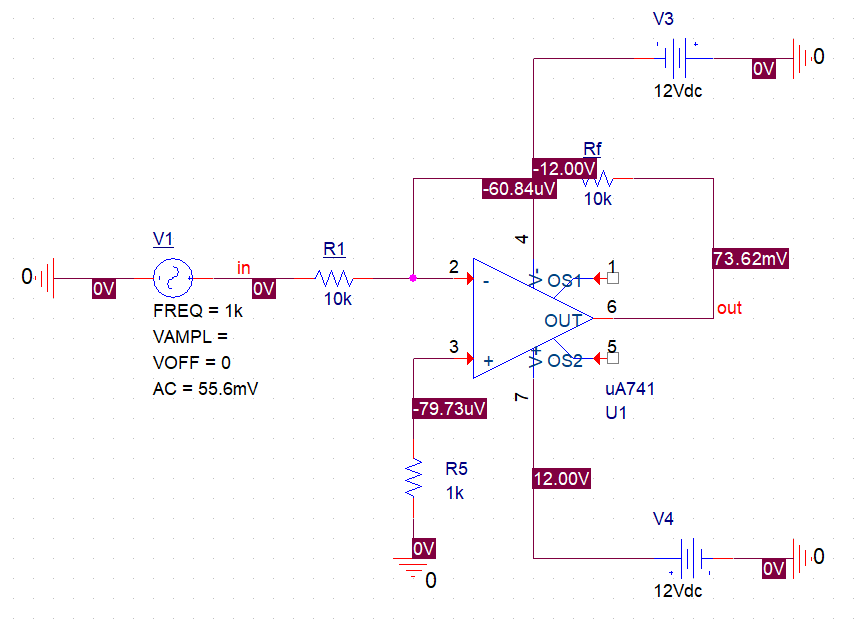
\includegraphics[width = 3in]{运算15}
                \caption{电路图}
            \end{figure}
            结果如下:
            \begin{table}[h]
                \centering
                \begin{tabular}{|c|c|c|c|c|c|}
                \hline
                \multicolumn{2}{|c|}{$R_f$} & $R_1$       & $A_v$ & $BW$     & $A_v \dot BW$ \\ \hline
                1       & $10k\Omega$       & $10k\Omega$ & 1.0 & $654.424kHz$ & $654.424kHz$      \\ \hline
                2       & $100k\Omega$      & $10k\Omega$ & 10.0    & $94.460kHz$  & $944.60kHz$      \\ \hline
                3       & $1M\Omega$        & $10k\Omega$ & 99.94  & $9.810kHz$ & $980.41kHz$   \\ \hline
                \end{tabular}
                \caption{仿真结果}
                \end{table}
    \section{实验结果和分析处理}
        \subsection{反相放大器}
        从直流和交流结果来看,反相放大器的增益基本达到设计要求$|A_v| = 10$,同时,从示波器的结果来看,输入输出信号的相位相同。
        \subsection{算术运算器}
        从实验得到的幅度来看,满足设计要求:
        $$v_o = -(v_{i1} + \frac{1}{2}v_{i2})$$
        同时仿真的结果图也和实验的结果相符合。
        \subsection{增益带宽积研究} 
        从实验的结果来看,当增益越高时,带宽越窄,同时增益带宽积在误差允许范围内基本等于常数。
        从仿真结果来看,也满足增益越高时,带宽越窄,同时误差允许范围内增益带宽积为常数。
    \section{讨论、心得}
        通过本次实验,我对集成运放电路的基本运算电路的组成和功能有了更加深入的理解和掌握。学会了其设计方法。
        同时通过对放大电路的增益带宽积的研究,了解了增益带宽积的特点。
\end{document}